\bab{METODE}
Tahapan penelitian terdiri atas lima tahap, yaitu: pengumpulan data email, ekstraksi dokumen email, praproses, membuat fungsi klasifikasi, dan evaluasi hasil. Gambar 1 menunjukkan diagram alir penelitian yang dilakukan.
\begin{figure*}[h!]
	\centering
	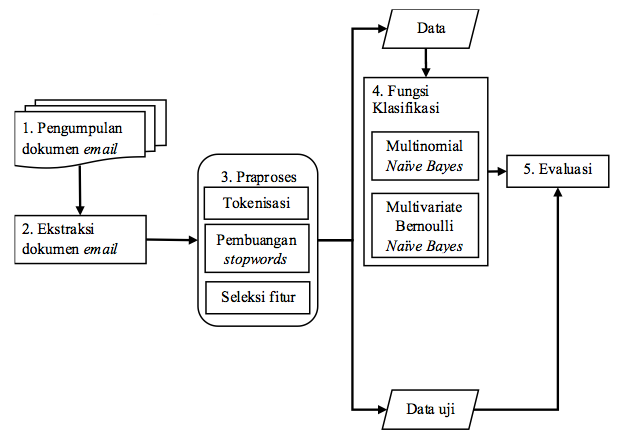
\includegraphics[width=400pt]{skemapenelitian.png}
	\caption{Diagram Alir Penelitian}
	\label{fig:skemapenelitian}
\end{figure*}

\subbab{Pengumpulan Dokumen Email}
Tahapan penelitian yang pertama adalah pengumpulan dokumen email. Dokumen email yang terkumpul digunakan sebagai korpus. Korpus yang digunakan pada penelitian ini adalah public email copus yang disediakan oleh Spamassasin\footnote{Diunduh dari  https://spamassassin.apache.org/publiccorpus/} dengan kode prefix “20030228”. Korpus email dibagi menjadi dua kelas yaitu kelas spam dan kelas ham. Korpus tersebut akan digunakan sebagai data latih dan data uji pada tahap selanjutnya.

\subbab{Ekstraksi Dokumen Email}
Dokumen email yang terdapat dalam korpus masih dengan format standar email yang terdiri dari header dan body. Oleh karena itu, struktur email tersebut harus dipecah sesuai dengan bagian-bagiannya. Ekstraksi dokumen email dilakukan untuk mendapatkan bagian email yang akan dimasukkan dalam proses tokenisasi. Tabel \ref{tab:strukturemail} menampilkan struktur yang terdapat dalam dokumen email. Bagian header yang digunakan untuk proses tokensisasi adalah subject, sedangkan pada bagian body adalah plain text dan HTML text.
\begin{table*}[h!]
	\begin{center}
		\caption{Struktur dokumen email}
		\label{tab:strukturemail}
		\small
		\begin{tabular}{l p{3cm} p{8cm}}
			\hline
			Bagian&Nama Struktur&Definisi\\
			\hline
			Header&MIME-version&Menunjukkan versi MIME yang digunakan\\
			&From&Nama dan alamat pengirim pesan\\
			&Received&Daftar semua server/komputer dimana pesan dapat sampai kepada penerimanya\\
			&Date&Menunjukkan tanggal dan waktu pesan email dibuat\\
			&Delivered-To&Alamat penerima email\\
			&Message-ID&Sebuah string unik yang diberikan oleh sistem mail saat pesan tersebut pertama kali dibuat\\
			&Subject To&Subjek dari pesan\\
			&To&Alamat yang mengirim pesan\\
			&X-Mailer&Aplikasi yang mengirimkan pesan\\
			&Return-Path&Alamat pengembalian pesan jika alamat penerima tidak ditemukan\\
			\hline
			Body&Plain text&Isi pesan dengan format penulisan dalam teks ASCII biasa\\
			&HTML text&Isi pesan yang mengandung tag HTML\\
			&Attachment&Informasi yang memberikan lampiran dari sebuah pesan\\
			\hline
		\end{tabular}
		\normalsize
	\end{center}
\end{table*}

\subbab{Praproses}
Dokumen email yang telah diekstraksi kemudian ditokenisasi. Tokenisasi adalah memotong dokumen teks menjadi potongan-potongan kecil yang disebut token dan membuang karakter-karakter tertentu seperti tanda baca (\cite{MANNING}). Whitespace (spasi, tab, newline) digunakan sebagai pemisah antar kata yang akan dipotong. Selain itu token yang dihasilkan biasanya diubah ke dalam bentuk lowercase. Proses tokensisasi dilakukan sebagai berikut:
\begin{itemize}
	\item Tanda baca diganti menjadi spasi sehingga tanda baca tersebut dianggap sebagai pemisah token. Tanda baca yang digunakan yaitu \'~- ) ( \textbackslash~ / = . , : ; ! ?.
	\item Teks dipotong menjadi token-token. Karakter numerik dibuang sehingga token hanya terdiri dari karakter huruf (string).
	\item Token dengan panjang kurang dari 3 karakter dibuang.
	\item Semua token diubah ke dalam bentuk lowercase.
\end{itemize}

Token yang termasuk ke dalam stopword\footnote{http://jmlr.org/papers/volume5/lewis04a/a11-smart-stop-list/english.stop} akan dibuang. Stopword adalah kata yang sangat umum dan sering muncul seperti kata sambung (\cite{MANNING}). Stopword tidak menambah informasi untuk fungsi klasifikasi dan untuk mengurangi beban komputasi.

Seleksi fitur merupakan suatu proses memilih subset dari setiap kata unik yang ada di dalam himpunan dokumen latih yang akan digunakan sebagai fitur di dalam klasifikasi dokumen. Subset kata unik yang terpilih disebut dengan penciri. Seleksi fitur memiliki dua tujuan, yaitu mengurangi jumlah kata yang digunakan dan meningkatkan akurasi hasil klasifikasi (\cite{MANNING}).

Pada penelitian ini, pemilihan fitur dilakukan dengan metode chi-square. Chi-square digunakan untuk menguji independensi antara dua kejadian yaitu kejadian kemunculan kata unik dan kejadian kemunculan kelas (\cite{MANNING}). Nilai chi-square kata t pada kelas c dihitung menggunakan persamaan:
\begin{equation}
	\label{eq:chisquare}
	\chi^2(t,c)=\sum_{e_t\in \{0,1\}}\sum_{e_c\in \{0,1\}}
	\frac{ [ N(e_te_c)-E(e_te_c) ]^2}{E(e_te_c)}
\end{equation}
\noindent dengan $N$ adalah frekuensi yang diamati dan $E$ adalah frekuensi yang diharapkan. Pada persamaan (\ref{eq:chisquare}), $e_t$ bernilai 1 jika dokumen mengandung kata $t$ dan $e_t$ bernilai 0 jika dokumen tidak mengandung kata $t$, sedangkan $e_c$ bernilai 1 jika dokumen terdapat dalam kelas $c$ dan $e_c$ bernilai 0 jika dokumen tidak terdapat dalam kelas $c$.
\begin{table*}[h!]
	\begin{center}
		\caption{Tabel kontingensi}
		\label{tab:kontingensi}
		\begin{tabular}{c c c}
			\hline
			\multirow{2}{*}{~~~~~Kata~~~~~}&\multicolumn{2}{c}{~~~~~~~~Kelas~~~~~~~~} \\
			\cline{2-3}
			&~~~$c$~~~&~~~$\neg c$~~~\\
			\hline
			$t$&A&B\\
			$\neg t$&C&D\\
			\hline
		\end{tabular}
	\end{center}
\end{table*}

Penghitungan nilai chi-square pada setiap kata $t$ yang muncul pada setiap kelas $c$ dapat dibantu dengan menggunakan tabel kontingensi (Tabel \ref{tab:kontingensi}). Nilai yang terdapat pada Tabel \ref{tab:kontingensi} merupakan nilai frekuensi obsevasi dari suatu kata terhadap kelas yaitu $A$ merupakan banyaknya dokumen pada kelas $c$ yang memuat kata $t$, $B$ merupakan banyaknya dokumen yang bukan kelas $c$ namun memuat kata $t$, $C$ merupakan banyaknya dokumen yang ada di kelas $c$ namun tidak memiliki kata $t$, serta $D$ merupakan banyaknya dokumen yang bukan kelas $c$ dan tidak memuat kata $t$.

Berdasarkan Tabel \ref{tab:kontingensi}, perhitungan chi-square pada (\ref{eq:chisquare}) dapat disederhanakan menjadi:
\begin{equation*}
	\label{eq:chisimple}
	\chi^2(t,c)=\frac{N(AD-BC)^2}{(A+C)(A+B)(B+D)(C+D)}
\end{equation*}
\noindent dengan $t$ merupakan kata yang diujikan terhadap suatu kelas $c$ dan $N$ merupakan jumlah dokumen latih.
\begin{table*}[h!]
	\begin{center}
		\caption{Nilai Kritis $\chi^2$}
		\label{tab:nilaikritis}
		\begin{tabular}{l r}
			\hline
			Taraf Nyata $(\alpha)$&Nilai Kritis\\
			\hline
			0.050&3.841\\ 
			0.025&5.024\\
			0.010&6.635\\
			0.005&7.879\\
			\hline
		\end{tabular}
	\end{center}
\end{table*}

Pengambilan keputusan dilakukan berdasarkan nilai $\chi^2$ dari masing-masing kata. Kata yang memiliki nilai $\chi^2$ lebih besar dari nilai kritis pada taraf nyata $\alpha$ adalah kata yang akan dipilih sebagai penciri dokumen. Kata yang dipilih sebagai penciri merupakan kata yang memiliki pengaruh terhadap kelas $c$. Nilai kritis $\chi^2$ untuk taraf nyata $\alpha$ (\cite{WALPOLE}) ditunjukkan pada Tabel \ref{tab:nilaikritis}.

Penelitian ini menggunakan satu taraf nyata $\alpha$ dengan nilai 0.01 yang diartikan bahwa kriteria kata yang dipilih sebagai penciri dokumen adalah kata yang memiliki nilai $\chi^2$ lebih besar dari 6.635. Hasil seleksi fitur ini akan digunakan sebagai vocabulary untuk proses klasifikasi.

\subbab{Fungsi Klasifikasi}
Ada dua cara mengelompokkan dokumen ke dalam kategori tertentu, yaitu manual dan otomatis. Cara pertama yaitu secara manual yang dilakukan oleh para pakar/ahli. Akan tetapi cara manual sulit dilakukan untuk dokumen dengan skala besar. Cara kedua adalah klasifikasi dokumen secara otomatis menggunakan fungsi klasifikasi yang dapat memetakan dokumen ke dalam kategori tertentu, $\gamma:\mathbb{X}\mapsto \mathbb{C}$, dengan $\mathbb{X}$ adalah kumpulan dokumen dan $\mathbb{C}$ adalah himpunan kelas atau kategori.

\citename{MANNING} membagi fungsi klasifikasi menjadi dua metode, yaitu metode berbasis vektor dan peluang. Pada fungsi klasifikasi berbasis vektor, setiap dokumen direpresentasikan sebagai vektor yang diberi label sesuai dengan kelasnya. Beberapa metode yang sering digunakan untuk klasifikasi berbasis vektor adalah kNN dan Rocchio classification.

Metode kedua adalah berbasis peluang dimana penentuan label kelas akan ditentukan dari nilai peluang dokumen terhadap kelas. Metode berbasis peluang yang sering digunakan adalah NB classifier. NB classifier terbagi menjadi dua model, yaitu Multivariate Bernoulli dan Multinomial NB.

Multivariate Bernoulli menyatakan bahwa dokumen diwakili oleh atribut biner yang menunjukkan ada dan tidak ada term dalam dokumen. Frekuensi kemunculan term dalam dokumen tidak ikut diperhitungkan. Ketika menghitung peluang dari sebuah dokumen, semua nilai atribut dikalikan termasuk kemungkinan ada dan tidak ada term dalam dokumen. Pada model ini, dokumen akan direpresentasikan ke dalam angka biner 1 jika terdapat dalam dokumen atau 0 jika tidak terdapat dalam dokumen:
\begin{equation*}
	d=<e_1, \dots, e_i, \dots e_M >, e_i\in \{0,1\}
\end{equation*}
\noindent Peluang dokumen $d$ dalam kelas $c$ dihitung menggunakan cara:
\begin{equation}
	\label{eq:peluangNBbernoulli}
	P(c|d)\propto \hat{P}(c)\prod_{t_i\in \mathbb{V}}\hat{P}(U_i=e_i|c)
\end{equation}
\noindent dengan $\hat{P}(U_i=e_i|c)$ adalah rasio dokumen dari kelas $c$ yang mengandung term $U_i$, $\hat{P}(c)$ adalah peluang dokumen pada kelas $c$. Pendugaan $\hat{P}(c)$ dan $\hat{P}(e_i|c)$ dihitung dengan cara:
\begin{equation*}
	\hat{P}(c)=\frac{N_c}{N},\xspace 
	\hat{P}(e_i|c)=\frac{T_{ct}}{\sum_{t\in V}T_{ct}}
\end{equation*}
\noindent dengan $T_{ct}$ adalah banyaknya dokumen yang mengandung term $t$ dalam dokumen latih kelas $c$. Untuk menghilangkan dugaan $\hat{P}(e_i|c)$ yang bernilai nol, digunakan Laplace smoothing atau Add-One Smoothing sehingga pendugaan $\hat{P}(e_i|c)$ menjadi:
\begin{equation}
	\label{eq:laplaceBernoulli}
	\hat{P}(e_i|c)=\frac{T_{ct}+1}{\sum_{t\in V}T_{ct}+b}
\end{equation}
\noindent dengan $b$ adalah banyaknya kelas atau kategori (\cite{MANNING}).

Dalam Multinomial NB, dokumen diwakili oleh serangkaian kemunculan term dari dokumen, yaitu:
\begin{equation*}
d=<t_1, \dots, t_k, \dots t_{n_d} >, t_k\in \mathbb{V}
\end{equation*}
\noindent Dalam model ini jumlah kemunculan dari setiap term dalam dokumen akan diperhitungkan. Peluang dokumen $d$ dalam kelas $c$ dihitung menggunakan persamaan:
\begin{equation}
\label{eq:peluangNBmultinom}
P(c|d)\propto \hat{P}(c)\prod_{1\leq k\leq n_d}\hat{P}(X=t_k|c)
\end{equation}
\noindent dengan $\hat{P}(X=t_k|c)$ adalah rasio term dalam kelas $c$ yang mengandung term $t$, $\hat{P}(c)$ adalah peluang dokumen pada kelas $c$. Pendugaan $\hat{P}(X=t_k|c)$ menggunakan Laplace smoothing yang dihitung dengan cara:
\begin{equation}
\label{eq:laplaceMultinom}
\hat{P}(t_k|c)=\frac{T_{ct}+1}{\sum_{t\in V}T_{ct}+b'}
\end{equation}
\noindent sedangkan $b'$ adalah banyaknya term dalam vocabulary.

\subbab{Evaluasi}
Langkah terakhir adalah melakukan pengujian dan evaluasi terhadap model klasifikasi yang telah dibuat. Pengujian dilakukan terhadap data uji yang telah ditentukan sebelumnya. Confussion Matrix (Tabel \ref{tab:confusionKelas}) digunakan untuk membantu perhitungan evaluasi dengan TP adalah banyaknya dokumen yang kelas aktualnya adalah kelas Spam dengan kelas prediksinya kelas Spam, FN adalah banyaknya dokumen yang kelas aktualnya adalah kelas Spam dengan kelas prediksinya kelas Ham, FP adalah banyaknya dokumen yang ada kelas aktualnya adalah kelas Ham dengan kelas prediksinya kelas Spam serta TN adalah banyaknya dokumen yang ada kelas aktualnya adalah kelas Ham dengan kelas prediksinya kelas Ham.
\begin{table*}[h!]
	\begin{center}
		\caption{Confussion Matrix kelas prediksi dan aktual}
		\label{tab:confusionKelas}
		\begin{tabular}{l c c}
			\hline
			\multirow{2}{*}{Kelas Aktual~~~~~~~~~~}&\multicolumn{2}{c}{Kelas Prediksi} \\
			\cline{2-3}
			&~~~~~Spam~~~~~&~~~~~Ham~~~~~\\
			\hline
			Spam&TP&FP\\
			Ham&FN&TN\\
			\hline
		\end{tabular}
	\end{center}
\end{table*}

\noindent Evaluasi penelitian ini menggunakan perhitungan akurasi dengan formula:
\begin{equation*}
	Akurasi=\frac{TP+TN}{TP+FN+FP+TN}
\end{equation*}

Untuk mengetahui akurasi setiap kelas digunakan perhitungan akurasi ham dan akurasi spam dengan formula:
\begin{equation*}
Akurasi~Ham=\frac{|H_k|}{|H|},~~Akurasi~Sam=\frac{|S_k|}{|S|}
\end{equation*}
\noindent dengan $|H_k|$ adalah banyaknya dokumen ham yang benar diklasifikasikan, $|H|$ adalah total dokumen ham, $|S_k|$ adalah banyaknya dokumen spam yang benar diklasifikasikan, dan $|S|$ adalah total dokumen spam.

Masing-masing model NB akan dihitung nilai akurasinya kemudian dibandingkan sehingga diketahui model mana yang paling baik untuk spam filter. Perbandingan model klasifikasi sebelum menggunakan seleksi fitur dan setelah menggunakan seleksi fitur dihitung untuk mengetaui pengaruh seleksi fitur terhadap model klasifikasi.

\subbab{Lingkungan Pengembangan}
Spesifikasi perangkat keras dan perangkat lunak yang digunakan untuk penelitian ini adalah sebagai berikut:
\begin{enumerate}
	\item Perangkat keras berupa komputer personal dengan spesifikasi sebagai berikut:
	\begin{itemize}
		\item Processor Intel Dual Core
		\item RAM 3GB
		\item Monitor LCD 14.0" HD
		\item Harddisk 250 GB HDD
	\end{itemize}
	\item Perangkat lunak:
	\begin{itemize}
		\item Sistem Operasi Windows 7
		\item Bahasa pemrograman PHP
		\item XAMPP v3.2.1
		\item Notepad++ digunakan sebagai editor kode program
	\end{itemize}
\end{enumerate}

